% shared preamble of the theory figures (white background, purple / black theme, sans-serif)
\documentclass[tikz,border=8pt]{standalone}
\usepackage[T1]{fontenc}
\usepackage[scaled=0.92]{helvet}
\renewcommand{\familydefault}{\sfdefault}
\usepackage{amsmath,amssymb}
\usepackage[helvet]{sfmath}
\usetikzlibrary{arrows.meta,calc,decorations.pathreplacing,positioning,backgrounds}
\definecolor{ink}{HTML}{1A1A1F}
\definecolor{cohesin}{HTML}{6A3DE8}
\definecolor{condensin}{HTML}{1BAF7A}
\definecolor{fwd}{HTML}{D1303F}      % CTCF pointing right
\definecolor{rev}{HTML}{2B62D9}      % CTCF pointing left
\definecolor{panel}{HTML}{F8F6FD}
\definecolor{panelline}{HTML}{E3DDF5}
\tikzset{
  fiber/.style={line width=2.1pt,ink,line cap=round,line join=round},
  halo/.style={line width=6pt,white,line cap=round},
  lab/.style={font=\small,text=ink},
  note/.style={font=\footnotesize,text=ink!60},
  hd/.style={font=\bfseries\small,text=ink,anchor=west},
  leader/.style={line width=0.6pt,ink!45},
}
% soft panel, numbered badge, heading
\newcommand{\panelbg}[4]{\draw[rounded corners=9pt,fill=panel,draw=panelline,line width=0.9pt] (#1,#2) rectangle (#3,#4);}
\newcommand{\badge}[3]{\fill[ink] (#1,#2) circle (0.21);\node[white,font=\bfseries\footnotesize] at (#1,#2) {#3};}
% CTCF: a protein on the fibre carrying an arrow that gives the motif direction (f = right, r = left)
\newcommand{\protf}[2]{\draw[rounded corners=3.5pt,line width=0.6pt,draw=fwd!65!black,fill=fwd] (#1-0.3,#2-0.19) rectangle (#1+0.3,#2+0.19);
  \draw[white,line width=1.5pt,-{Stealth[length=3.4pt,width=4.4pt]}] (#1-0.15,#2)--(#1+0.16,#2);}
\newcommand{\protr}[2]{\draw[rounded corners=3.5pt,line width=0.6pt,draw=rev!65!black,fill=rev] (#1-0.3,#2-0.19) rectangle (#1+0.3,#2+0.19);
  \draw[white,line width=1.5pt,-{Stealth[length=3.4pt,width=4.4pt]}] (#1+0.15,#2)--(#1-0.16,#2);}
\newcommand{\prot}[3]{\csname prot#3\endcsname{#1}{#2}}
% ring seen at an angle, drawn as a tube (dark outline, light core); back half and front half
\newcommand{\ringpart}[5]{\draw[line width=4.6pt,#3!80!black,line cap=round] ([shift={(#1,#2)}]#4:0.55 and 0.21) arc[start angle=#4,end angle=#5,x radius=0.55,y radius=0.21];
  \draw[line width=2.4pt,#3!55!white,line cap=round] ([shift={(#1,#2)}]#4:0.55 and 0.21) arc[start angle=#4,end angle=#5,x radius=0.55,y radius=0.21];}
\newcommand{\ringback}[3]{\ringpart{#1}{#2}{#3}{180}{0}}
\newcommand{\ringfront}[3]{\ringpart{#1}{#2}{#3}{180}{360}}
% smooth loop whose foot (ring) is at (cx,y0): half-width W, height H, ring colour
\newcommand{\lloop}[5]{%
  \ringback{#1}{#2}{#5}%
  \draw[fiber] (#1-0.3,#2) .. controls (#1-0.3,#2+0.25*#4) and (#1-#3,#2+0.2*#4) .. (#1-#3,#2+0.55*#4)
     .. controls (#1-#3,#2+0.95*#4) and (#1-0.5*#3,#2+#4) .. (#1,#2+#4)
     .. controls (#1+0.5*#3,#2+#4) and (#1+#3,#2+0.95*#4) .. (#1+#3,#2+0.55*#4)
     .. controls (#1+#3,#2+0.2*#4) and (#1+0.3,#2+0.25*#4) .. (#1+0.3,#2);%
  \ringfront{#1}{#2}{#5}}
% gently undulating fibre from x0 to the loop foot at cx (height y0), and from x1
\newcommand{\base}[4]{%
  \draw[fiber] plot[smooth] coordinates {(#1,0.05) (#1+0.35*#3-0.35*#1,-0.05) (#3-1.4,0.04)} .. controls (#3-0.6,0.02) and (#3-0.3,0.05) .. (#3-0.3,#4);
  \draw[fiber] plot[smooth] coordinates {(#2,-0.05) (#2-0.35*#2+0.35*#3,0.05) (#3+1.4,-0.04)} .. controls (#3+0.6,-0.02) and (#3+0.3,0.05) .. (#3+0.3,#4);}
% stop sign for a blocked leg and a leg arrow
\newcommand{\stopbar}[3]{\draw[#3,line width=2.4pt,line cap=round] (#1,#2-0.2)--(#1,#2+0.2);}
\newcommand{\legarrow}[3]{\draw[cohesin,line width=1.6pt,-{Stealth[length=5pt,width=6pt]},line cap=round] (#1,#3)--(#2,#3);}

\tikzset{st/.style={rounded corners=7pt,draw=cohesin!70,fill=white,line width=0.9pt,minimum width=3.7cm,minimum height=2.0cm,align=center,font=\small,text=ink,inner sep=4pt},
  opt/.style={st,dashed,fill=cohesin!5},
  io/.style={st,draw=ink!55,fill=panel},
  ar/.style={line width=1.3pt,ink!65,-{Stealth[length=5.5pt,width=6.5pt]}}}
\newcommand{\cache}[1]{{\scriptsize\ttfamily\color{ink!55}#1}}
\begin{document}
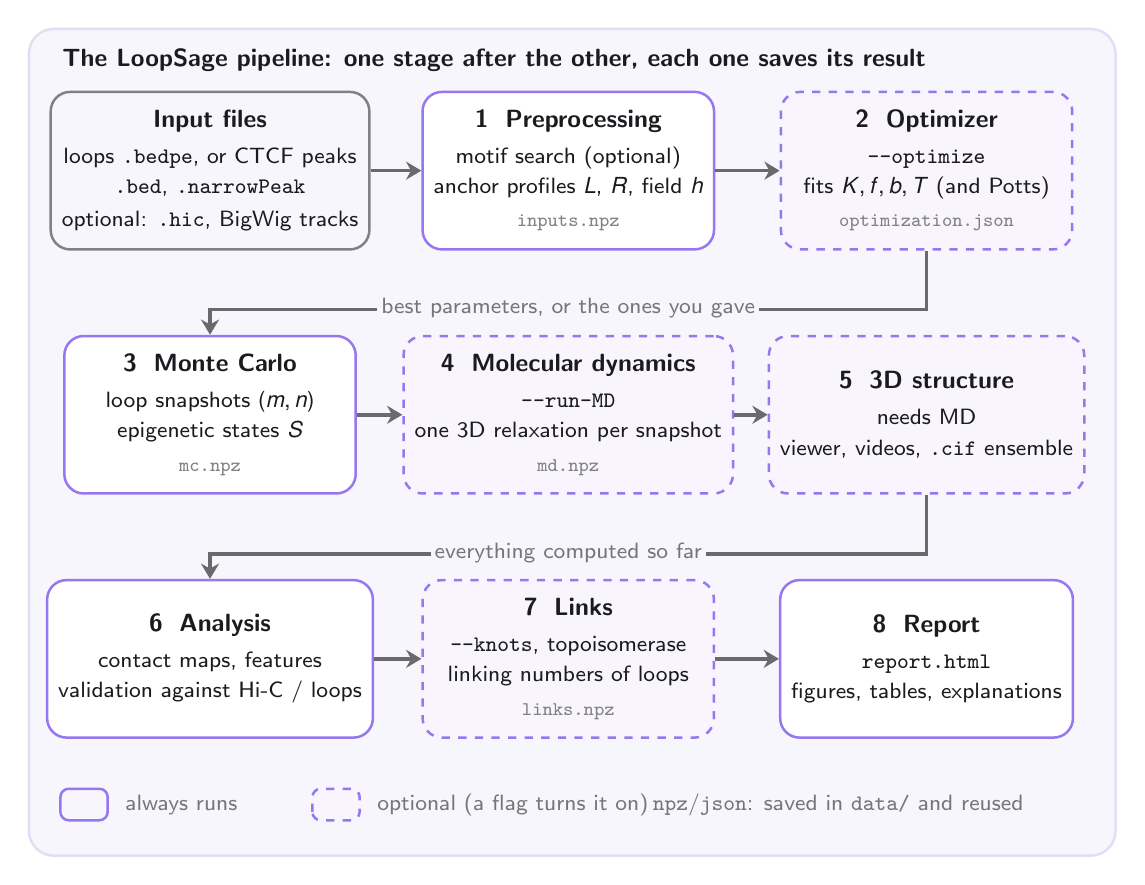
\begin{tikzpicture}
  \panelbg{-0.2}{-8.9}{13.6}{1.6}
  \node[hd] at (0.1,1.2) {The LoopSage pipeline: one stage after the other, each one saves its result};
  % row 1
  \node[io]  (inp)  at (2.1,-0.2)  {\bfseries Input files\\[2pt]{\footnotesize loops \texttt{.bedpe}, or CTCF peaks}\\{\footnotesize\texttt{.bed}, \texttt{.narrowPeak}}\\[1pt]{\footnotesize optional: \texttt{.hic}, BigWig tracks}};
  \node[st]  (pre) at (6.65,-0.2) {\bfseries 1\; Preprocessing\\[2pt]{\footnotesize motif search (optional)}\\{\footnotesize anchor profiles $L$, $R$, field $h$}\\[1pt]\cache{inputs.npz}};
  \node[opt] (op)  at (11.2,-0.2) {\bfseries 2\; Optimizer\\[2pt]{\footnotesize \texttt{-{}-optimize}}\\{\footnotesize fits $K, f, b, T$ (and Potts)}\\[1pt]\cache{optimization.json}};
  % row 2
  \node[st]  (mc)  at (2.1,-3.3)  {\bfseries 3\; Monte Carlo\\[2pt]{\footnotesize loop snapshots $(m,n)$}\\{\footnotesize epigenetic states $S$}\\[1pt]\cache{mc.npz}};
  \node[opt] (md)  at (6.65,-3.3) {\bfseries 4\; Molecular dynamics\\[2pt]{\footnotesize \texttt{-{}-run-MD}}\\{\footnotesize one 3D relaxation per snapshot}\\[1pt]\cache{md.npz}};
  \node[opt] (str) at (11.2,-3.3) {\bfseries 5\; 3D structure\\[2pt]{\footnotesize needs MD}\\{\footnotesize viewer, videos, \texttt{.cif} ensemble}};
  % row 3
  \node[st]  (an)  at (2.1,-6.4)  {\bfseries 6\; Analysis\\[2pt]{\footnotesize contact maps, features}\\{\footnotesize validation against Hi-C / loops}};
  \node[opt] (lk)  at (6.65,-6.4) {\bfseries 7\; Links\\[2pt]{\footnotesize \texttt{-{}-knots}, topoisomerase}\\{\footnotesize linking numbers of loops}\\[1pt]\cache{links.npz}};
  \node[st]  (rep) at (11.2,-6.4) {\bfseries 8\; Report\\[2pt]{\footnotesize \texttt{report.html}}\\{\footnotesize figures, tables, explanations}};
  \draw[ar] (inp)--(pre); \draw[ar] (pre)--(op);
  \draw[ar] (mc)--(md); \draw[ar] (md)--(str);
  \draw[ar] (an)--(lk); \draw[ar] (lk)--(rep);
  % wrap-around arrows
  \draw[ar] (op.south)--++(0,-0.75)-|(mc.north);
  \draw[ar] (str.south)--++(0,-0.75)-|(an.north);
  \node[note,fill=panel,inner sep=1.5pt] at (6.65,-1.95) {best parameters, or the ones you gave};
  \node[note,fill=panel,inner sep=1.5pt] at (6.65,-5.05) {everything computed so far};
  % legend
  \draw[rounded corners=3pt,draw=cohesin!70,line width=0.9pt] (0.2,-8.45) rectangle (0.8,-8.05);\node[note,anchor=west] at (0.9,-8.25) {always runs};
  \draw[rounded corners=3pt,draw=cohesin!70,dashed,line width=0.9pt,fill=cohesin!5] (3.4,-8.45) rectangle (4.0,-8.05);\node[note,anchor=west] at (4.1,-8.25) {optional (a flag turns it on)};
  \node[note,anchor=west] at (7.6,-8.25) {\texttt{npz}/\texttt{json}: saved in \texttt{data/} and reused};
\end{tikzpicture}
\end{document}
